\section{Architectural Design}
\subsection{Overview}
In Figure \ref{fig:three_layers_application} it's present the black-box view of our architecture, that is defined by three different layers represented:

\begin{itemize}
    \item \textbf{Presentation Layer:} it's the layer that is used to present data from the application layer in an accurate, well-defined and standardized format; in this case it is represented by the mobile application.
    \item \textbf{Application Layer:} it's the layer that manages all the functions that controls the business logic of our system (back-end).
    \item \textbf{Data Layer:} it controls how the data are stored and accessed (DB).
\end{itemize}

\begin{figure}[h!]
        \centering
        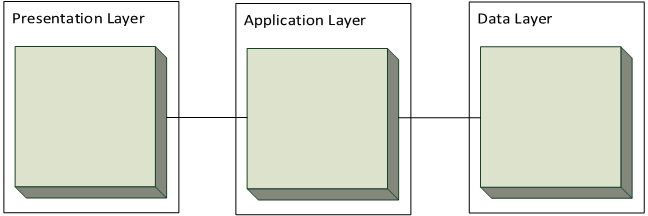
\includegraphics[scale=0.6]{images/three_layers.png}
        \caption{Three layers application}
        \label{fig:three_layers_application}
\end{figure}
\FloatBarrier

Generally, the architecture divide the application in three different layers: the user can interface with the mobile application which is connected to the application layer by means of RESTful API. The Application layer represents the back-end with the application logic and the Data layer is the the DBMS that provides (by DBMS APIs) the function to retrieve and store the data by the application server.
\newpage
\subsection{Deployment View}

\begin{figure}[h!]
        \centering
        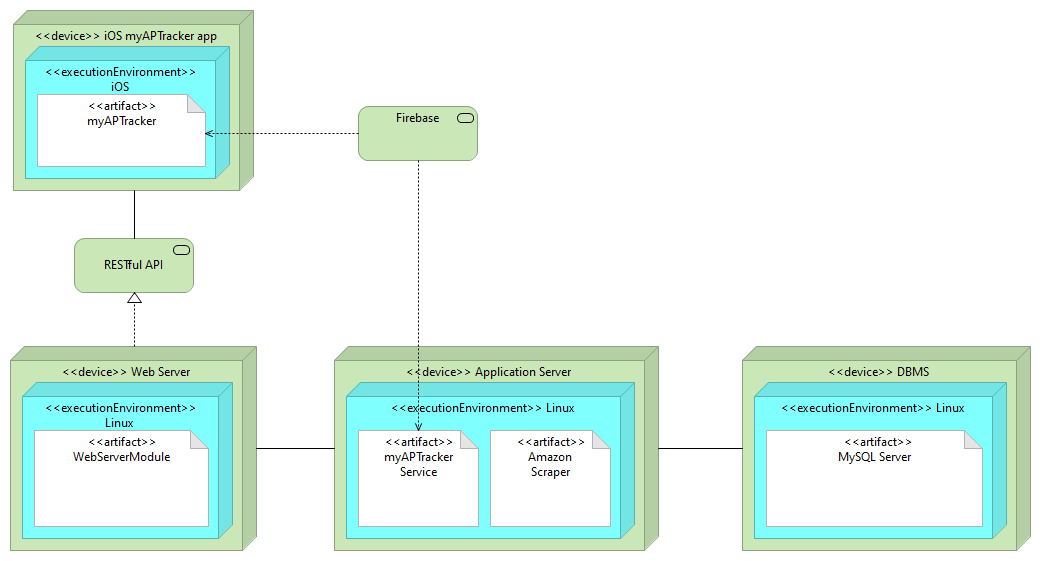
\includegraphics[scale=0.40]{images/deployment_view.png}
        \caption{Deployment Diagram}
        \label{fig:deployement_diagram}
\end{figure}
\FloatBarrier

The deployment diagram in figure \ref{fig:deployement_diagram} shows the topology of the system's hardware and specify the distribution of components. For each device its Operating System is indicated.
\begin{itemize}
    \item \textbf{Tier 1}: It is the client machine. It is an iPhone or and iPad where the application is installed.
    \item \textbf{Tier 2}: It consists in the web server that provides the RESTful APIs managing HTTP requests and forwarding them to the application server.
    \item \textbf{Tier 3}: it consists of the application servers. They provides all the business logic, allowing to manage requests and it is connect to the data tier using the DBMS gateway.
    \item \textbf{Tier 4}: it consists of the database management system servers. The data are stored in this device and it provide to the application server tier the operations needed to manage the data.
\end{itemize}
\newpage
\subsection{Runtime View}
\subsubsection{Local registration}

\begin{figure}[h!]
        \centering
        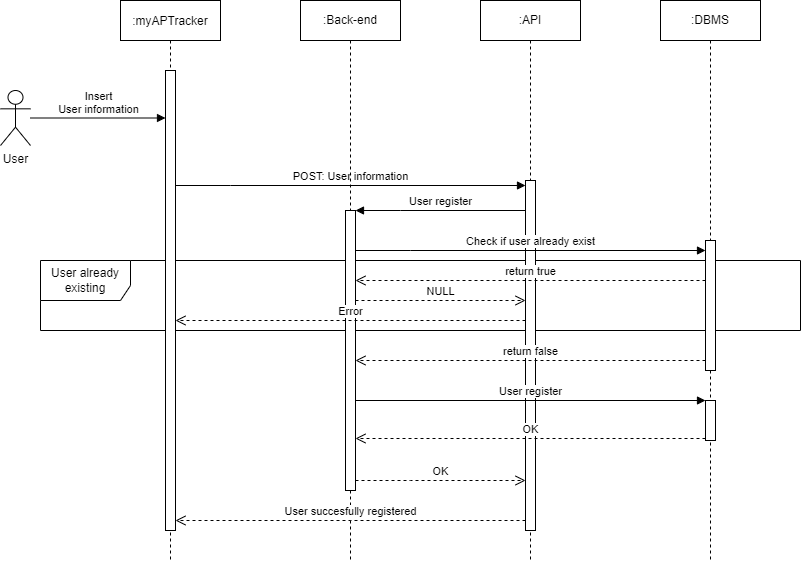
\includegraphics[scale=0.40]{images/runtime_view/local_registration.png}
        \caption{Local registration sequence diagram}
        \label{fig:local_registration_sequence_diagram}
\end{figure}
\FloatBarrier

This is the sequence diagram of a local registration done by a user. When registering, if the credentials inserted (email) are already stored in the DB an error will occur and it is returned to the application, otherwise the user data and the credential will be stored in the database and a success response is returned.
\newpage
\subsubsection{Local login}

\begin{figure}[h!]
        \centering
        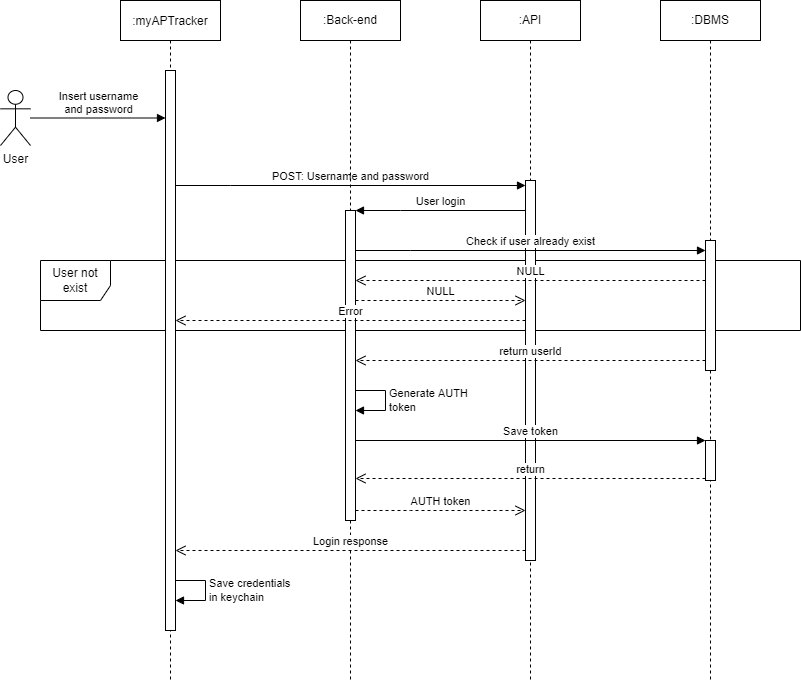
\includegraphics[scale=0.40]{images/runtime_view/local_login.png}
        \caption{Local login sequence diagram}
        \label{fig:local_login_sequence_diagram}
\end{figure}
\FloatBarrier

This is the sequence diagram of a local login done by a user. Before the login the user must be registered to the myAPTracker or an error will occur.
As a positive response of the login flow, an auth token and a refresh token are returned by the server. The refresh token is then used in order to require a new auth token when expired (the refresh flow is omitted since it is equal to the login one but the refresh token is sent instead of credential).
\newpage
\subsubsection{Social login - Google}

\begin{figure}[h!]
        \centering
        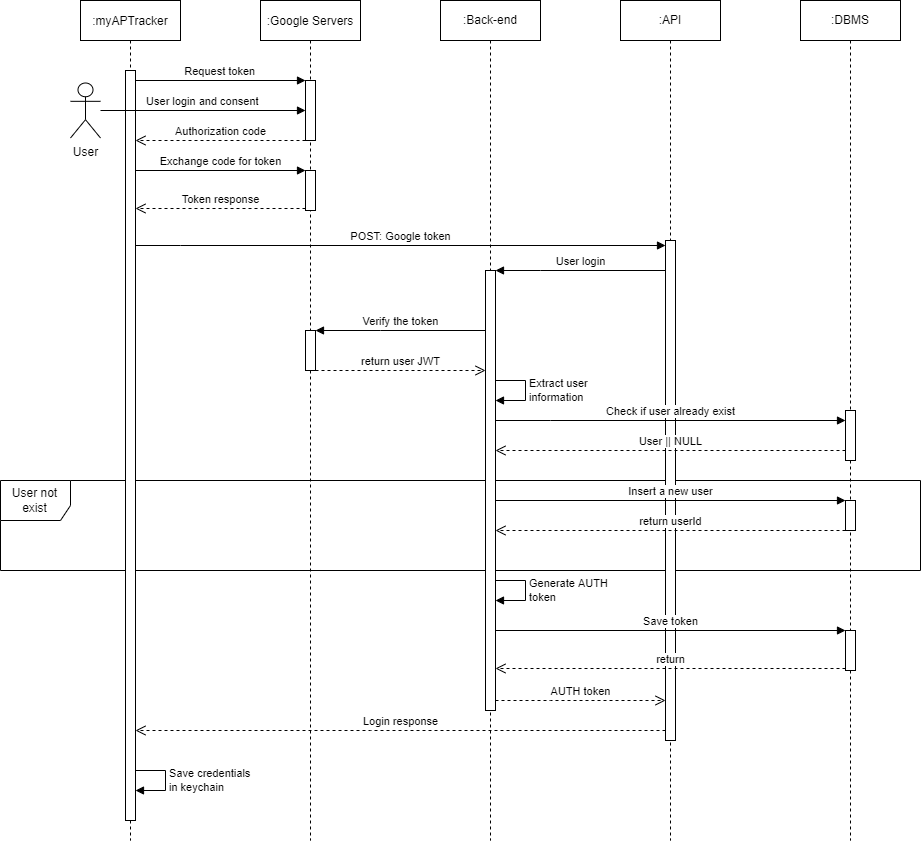
\includegraphics[scale=0.40]{images/runtime_view/social_login_google.png}
        \caption{Google Social login sequence diagram}
        \label{fig:google_social_login_sequence_diagram}
\end{figure}
\FloatBarrier

This is the sequence diagram of a login from a user that use Google as external service for the social authentication.\\
The flow can be considered the union of the registration and login ones. Once the application send the google token received by the social authentication, it is validated and then used to retrieve user data. If the user email is not present in the database the new user in inserted using the register function.
Finally, in both cases, the auth token and the refresh token are returned to the application.
\newpage
\subsubsection{Social login - Facebook}

\begin{figure}[h!]
        \centering
        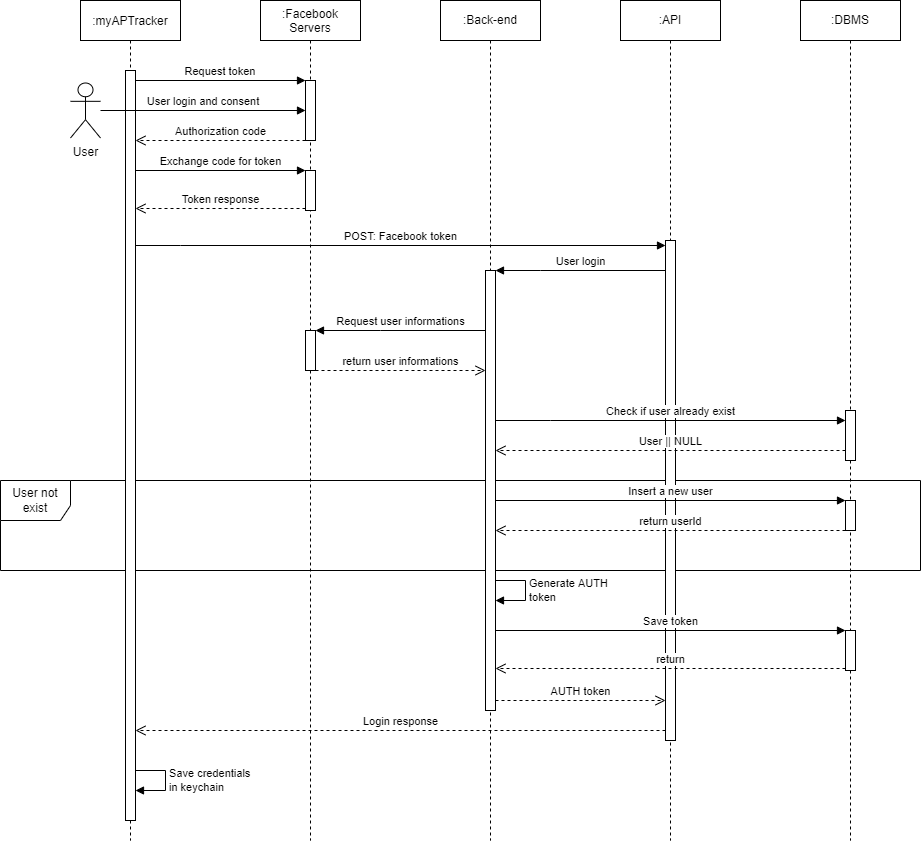
\includegraphics[scale=0.40]{images/runtime_view/social_login_facebook.png}
        \caption{Facebook Social login sequence diagram}
        \label{fig:facebook_social_login_sequence_diagram}
\end{figure}
\FloatBarrier

This is the sequence diagram of a login from a user that use Facebook as external service for the social authentication.\\
The flow is equal to Google's one.
\newpage
\subsubsection{Social login - Apple}

\begin{figure}[h!]
        \centering
        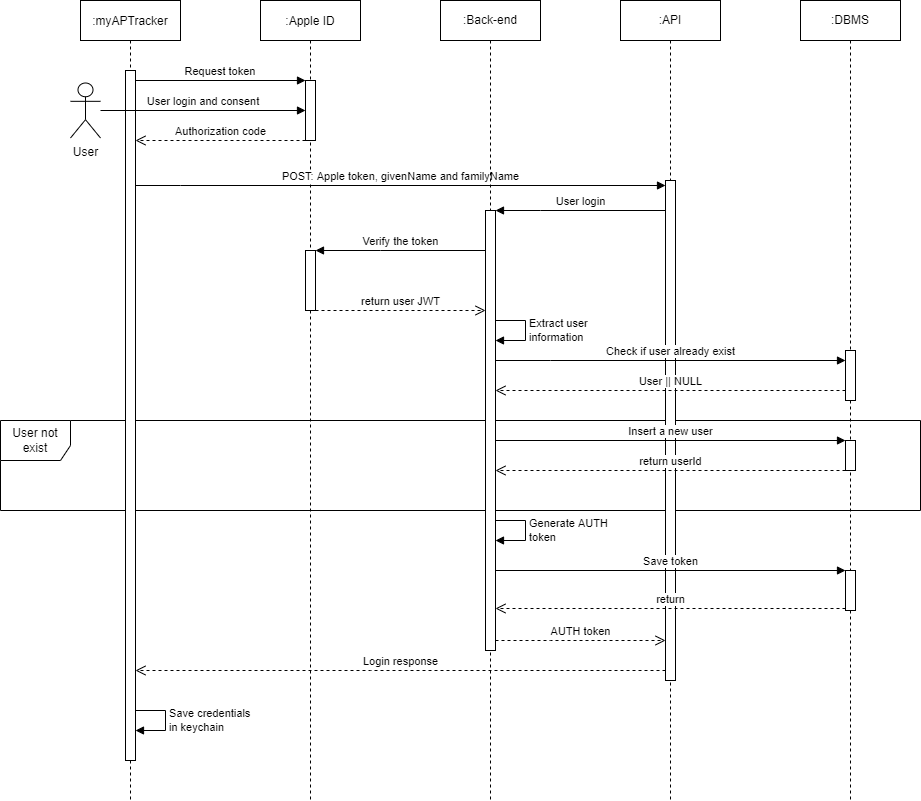
\includegraphics[scale=0.40]{images/runtime_view/social_login_apple.png}
        \caption{Apple Social login sequence diagram}
        \label{fig:apple_social_login_sequence_diagram}
\end{figure}
\FloatBarrier

This is the sequence diagram of a login from a user that use Apple as external service for the social authentication.\\
Very similar to the other social flows, Apple Sign-In requires also to send the user data (name and surname) since these data can be dynamically set by the user at the fist sign-in and they cannot be retrieved in a further moment. 

\newpage

\subsubsection{Track product}

\begin{figure}[h!]
        \centering
        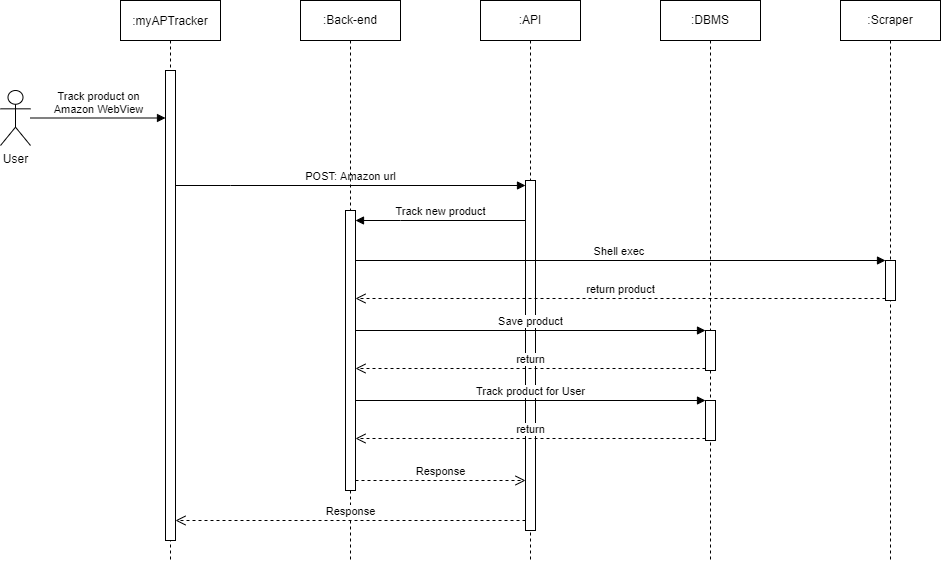
\includegraphics[scale=0.40]{images/runtime_view/track_product.png}
        \caption{Track product sequence diagram}
        \label{fig:track_product_sequence_diagram}
\end{figure}
\FloatBarrier

This is the sequence diagram when a user try to track a product. Once the application post the amazon URL to the endpoint, the server function calls the Scraper by shell execution it retrieves all the relevant information about the given product, storing them later on the DB. Finally, the product is marked as tracked in the database for the user who posts the URL.

\subsubsection{Generic API}

\begin{figure}[h!]
        \centering
        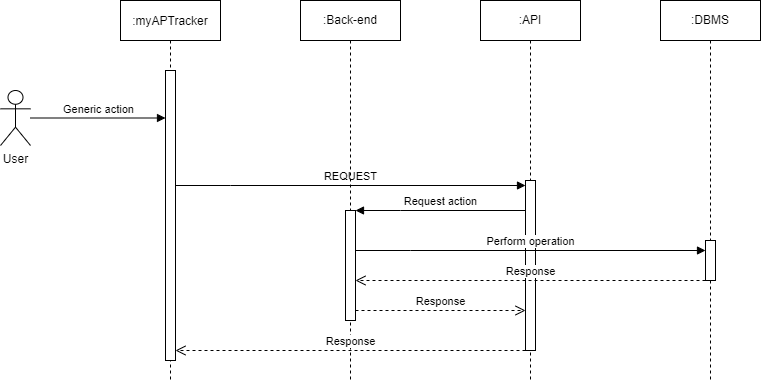
\includegraphics[scale=0.40]{images/runtime_view/generic_api.png}
        \caption{Generic API sequence diagram}
        \label{fig:generic_api_sequence_diagram}
\end{figure}
\FloatBarrier

This is the sequence diagram when a user do a generic action that involves the call of an API.
All the functionalities that require to communicate with the database make a request to the specific endpoint which calls the correspondent server function. The server communicate with the database to get/save/update the data and it returns a response to the application.

\subsubsection{Update price and notify users}

\begin{figure}[h!]
        \centering
        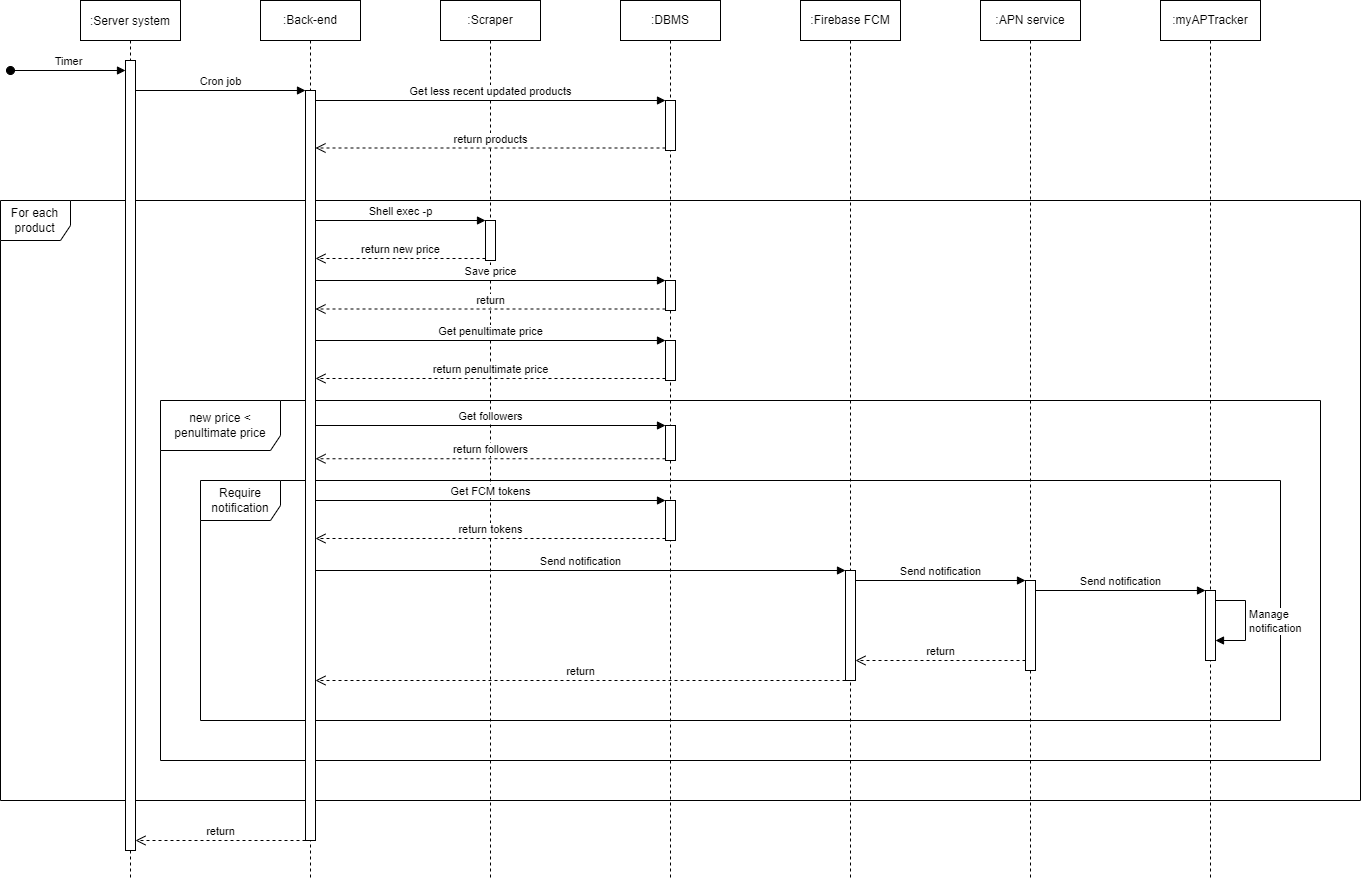
\includegraphics[scale=0.25]{images/runtime_view/update_notification.png}
        \caption{Update price and notify users sequence diagram}
        \label{fig:update_notification_sequence_diagram}
\end{figure}
\FloatBarrier

This is the sequence diagram when a user receive a notification for a product drop.
This flow is not invoked by a user action but, instead, by a cron-job scheduled in the server OS.\\
The server load all the products that need to be updated and for each of them calls (by shell execution) the Scraper (using --price-only flag) which returns the updated price the server now store in the database.
Then the server loads the penultimate price (since the new one is already saved) and if the new is lower then the previous one, all the user tracking it are taken.\\
Now each user could have a different notification setting so, for each one, the condition is checked and, if satisfied, the tokens of user devices are sent to Firebase Cloud Messaging (FCM) endpoint.\\
Finally, FCM is configured to forward notification to APN service which is responsible to send push notification to devices.

\newpage
\subsection{Logical Description of Data}

\begin{figure}[h!]
        \centering
        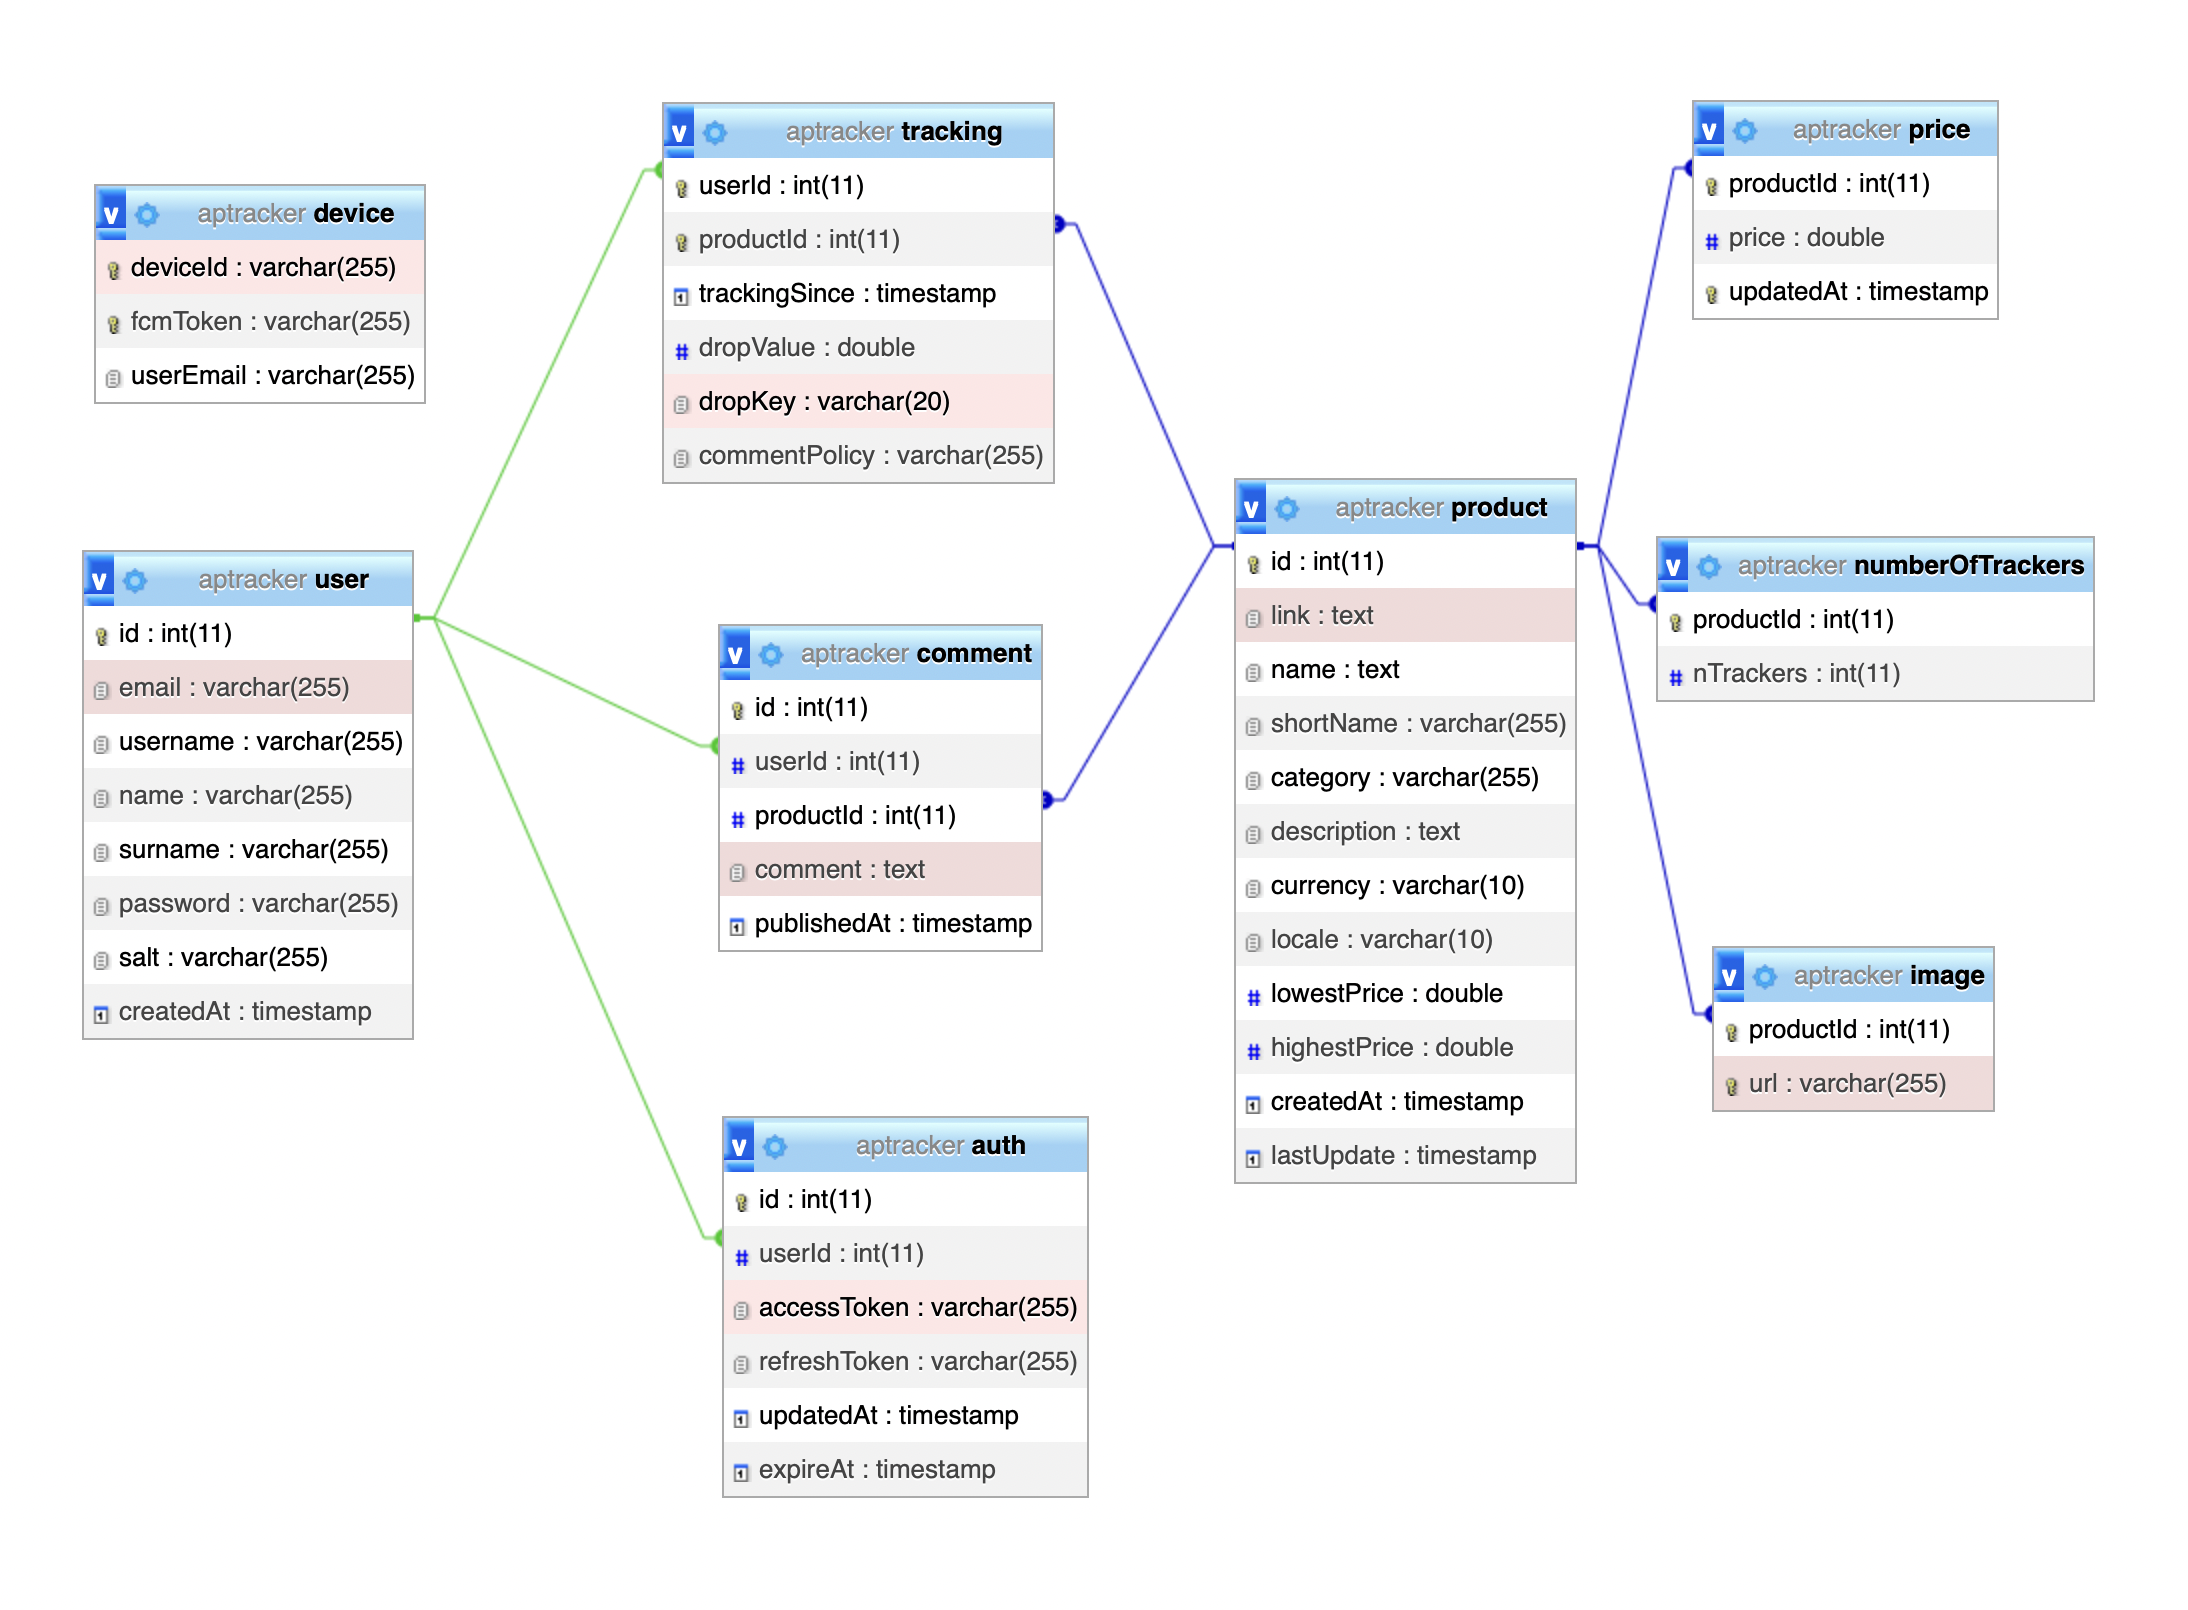
\includegraphics[scale=0.35]{images/er_diagrams/db_er.png}
        \caption{Back-end database ER diagram}
        \label{fig:er_diagram}
\end{figure}
\FloatBarrier

\begin{figure}[h!]
        \centering
        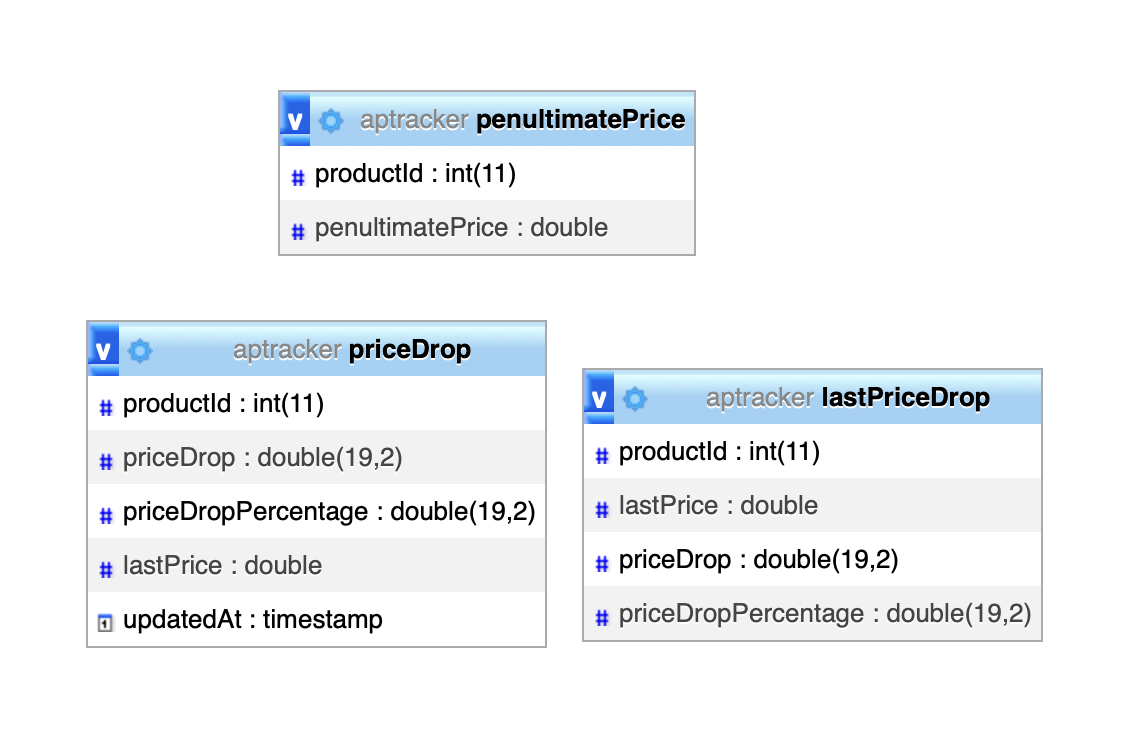
\includegraphics[scale=0.45]{images/er_diagrams/er_views.png}
        \caption{Useful Views in the DB}
        \label{fig:er_views}
\end{figure}
\FloatBarrier

The two figures above show the database structure used for our back-end and some useful views that we have used for retrieve some set of prices.\\
The database (fig: \ref{fig:er_diagram}) contains all the relevant information regarding the user and the product stored.
The \textit{user} table stores all the information created for a user when he registers while his authentication credentials (auth token, refresh token and expiration date) are stored in the \textit{auth} table.\\
The \textit{product} table contains the product information retrieved from the scraper with the \textit{image} table used to store the multiple images related to a product and the \textit{price} table for the product price history. The \textit{comment} table stores the comments a user post in a product page while the \textit{tracking} table keeps in relation a user with the tracked products. A \textit{numberOfTrackers} table is used to keep easily track of the number of trackers for each product and it is kept updated by triggers.\\
Finally, the \textit{device} table is responsible to keep the association of the device token with its FCM token and eventually, if a user is correctly logged in, the record is associated also with the user email.\\


The Views (fig: \ref{fig:er_views}) are used to get relevant data faster, in particular to get products in different orders. The most relevant API that require this views are: 
\begin{itemize}
    \item \textbf{GetByLastPriceDrop:} get the products ordered by the drop between the last two prices ordered by absolute drop.
    \item \textbf{GetByLastPriceDropPercentage:} get the products by the drop between the last two prices ordered by drop percentage.
    \item \textbf{GetByPriceDrop:} get the products by the drop between the highest and lowest price ordered by absolute drop.
    \item \textbf{GetByPriceDropPercentage:} get the products by the drop between the highest and lowest price ordered by drop percentage.
    \item \textbf{GetMostTracked:} get the product ordered by most tracked product.
\end{itemize}
For all those API also a correspondent paging function is present to allows the user to load less products and divide them in pages.

\subsection{Architectural Style and Patterns}
\subsubsection{Four-tiered architecture}
The usage of a four-tier architecture allows having four layers with completely different goals:
\begin{itemize}
    \item Presentation Layer (PL);
    \item Data Presentation Layer (DPL);
    \item Business Logic Layer (BLL);
    \item Data Access Layer (DAL).
\end{itemize}

Each tier is responsible for a specific layer: this implies that the logic is separated and changes at a certain tier, doing like that will not affect the other layers. This improves the maintainability of code and it is easier to implement new features.
\\This architectural style allows to improve security because users can not have direct access to database structure.\\ 
Finally, this division improve also the simplicity to add new feature and perform updates on the logic without changing the presentation layer.

\subsection{Model View View-Model (MVVM)}
Model-View-ViewModel (MVVM) is a software design pattern that is structured to separate program logic and user interface controls.\\
The separation of the code in MVVM is divided into View, ViewModel and Model:
\begin{itemize}
    \item \textbf{Model:} provides the logic for the program, which is retrieved by the ViewModel upon its own receipt of input from the user through the View.
    \item \textbf{View:} is the collection of visible elements, directly interactable by the user, which also receives user input. This includes user interfaces (UI), animations and text.
    \item \textbf{ViewModel:} is located between the View and Model layers. This is where the controls for interacting with the View are present and contains also the controls for modify the data present in the Model.
\end{itemize}
This pattern has been applied to the application.

\subsubsection{Model View Controller (MVC)}
Model-View-Controller is a software design pattern used for developing User interfaces that divides the related program logic into three interconnected elements. This is done to separate internal representations of information, from the ways information is presented to and accepted from the user.\\
These three components are:
\begin{itemize}
    \item \textbf{Model:} the central component of the pattern. It is the application's dynamic data structure, independent of the user interface. It directly manages the data, logic and rules of the application.
    \item  \textbf{View:} any representation of information such as the JSON output of the API interface. 
    \item  \textbf{Controller:} accepts input from the client and converts it to commands for the model that generally lead to state changes in the view.
\end{itemize} 
This pattern has been applied to the back-end.

\subsection{Other Design Decision}

\subsubsection{Easy usability}
Since our target is a customer of every age, the application is designed to be very simple and intuitive, so particular attention must be put on the organization on the interfaces following official Apple guideline taking care also to provide a device-dependent user interface.

\subsubsection{Security}
The application has an encrypted communication with the backend going on a secure channel using SSL protocol over HTTP (obtaining HTTPS) and also the application is integrated with social authentication (Apple, Facebook and Google) relying on OAuth2.0 protocol.
